\documentclass{ctexart}
% \usepackage[UTF-8]{ctex}
\usepackage{amsmath}
\usepackage{booktabs}
\usepackage{multirow}
\usepackage{tabularx}

\usepackage{booktabs,multirow,longtable}

\usepackage{listings}
\usepackage{listings}
\usepackage{color}

%导言区插入下面三行
\usepackage{graphicx} %插入图片的宏包
\usepackage{float} %设置图片浮动位置的宏包
\usepackage{subfigure} %插入多图时用子图显示的宏包


\definecolor{dkgreen}{rgb}{0,0.6,0}
\definecolor{gray}{rgb}{0.5,0.5,0.5}
\definecolor{mauve}{rgb}{0.58,0,0.82}

\lstset{frame=tb,
  language=Python,
  aboveskip=3mm,
  belowskip=3mm,
  showstringspaces=false,
  columns=flexible,
  basicstyle={\small\ttfamily},
  numbers=left,
  numberstyle=\tiny\color{gray},
  keywordstyle=\color{blue},
  commentstyle=\color{dkgreen},
  stringstyle=\color{mauve},
  breaklines=true,
  breakatwhitespace=true,
  tabsize=3
}


\title{作业3:数值求解热传导方程}
\author{谢文进}
\date{\today}
\begin{document}
\maketitle
\section{数值求解热传导方程}
\subsection{最简显格式}
对于如下热传导方程:
\begin{equation}
    \begin{cases}
        \frac{\partial u}{\partial t} =\frac{\partial ^2 u}{\partial t}  \quad 0<t<0.03,0<x<1 \\  
        u(x,0)=\sin(4\pi x) \quad 0 \le x \le 1 \\
        u(0,t)  = 0 \quad  0 \le t \le 0.03 \\
        u(1,t)  = 0 \quad 0 \le t \le 0.03
    \end{cases}
\end{equation}
该方程的精确解为$u(t,x)=e^{-(4\pi)^2t}\sin (4 \pi x),0\le t \le 0.03, 0 \le x \le 1.$

首先对时间及空间进行划分,将时间划分为$m-1$份,将空间划分为$n-1$份,则$\tau=\frac{0.03}{m-1},h=\frac{1}{n-1}$。
根据最简显格式可以得到:
\begin{equation}
    u_j^{i+1}=\frac{\tau}{h^2}(u_{j+1}^{i}-2u_j^i+u_{j-1}^i)+u_j^{i},
\end{equation}
其中$i=0,1,\cdots,m-1$,$j=0,1,\cdots,n-1$。
\subsection{编程实现}
根据理论推导,用python编写程序如下:
\begin{lstlisting}
    # -*- coding: utf-8 -*-
    """
    Created on Sun May 23 11:16:13 2021
    
    @author: XieWenjin
    """
    
    import math
    import numpy as np
    from matplotlib import pyplot as plt
    from mpl_toolkits.mplot3d import Axes3D
    
    t = 0.03     # 时间范围
    x = 1.0      # 空间范围
    m = input("请输入m:")
    m = int(m)
    n = input("请输入n:")
    n = int(n)
    # m = 320        # 时间方向分为320个格子
    # n = 64        # 空间方向的格子数
    dt = t / (m - 1)  # 时间步长
    dx = x / (n - 1)  # 空间步长
     
    def generate_u(m,n):
        u = np.zeros([m,n])
        # 边界条件
        for j in range(n):
            u[0,j] = math.sin(4 * math.pi * j * dx)
        for i in range(m):
            u[i,0] = 0
            u[i,-1] = 0
    
        # 差分法
        for i in range(m - 1):
            for j in range(1,n - 1):
                u[i+1, j] = dt * (u[i, j + 1] + u[i, j - 1] - 2 * u[i, j]) / dx ** 2 + u[i, j]
        return u
    
    def drawing(X,Y,Z):
        fig = plt.figure()
        ax = Axes3D(fig)
        ax.plot_surface(X, Y, Z, rstride=1, cstride=1, cmap='rainbow')
        plt.show()
    
    def error(u,u_exact):
        err = abs(u - u_exact)
        return max(map(max, err))
    
    X = np.arange(0, t + dt, dt) # remark:t+dt,not t
    Y = np.arange(0, x + dx, dx)
    X, Y = np.meshgrid(X, Y)
    u_exact = np.exp(- (4*np.pi)**2*X)*np.sin(4*np.pi*Y)
    
    u = generate_u(m,n)
    u = np.transpose(u) # 注意这里是转置,而不是np.reshape(u,(n,m))
    
    # print(m,n)
    print(error(u,u_exact))
    
    drawing(X,Y,u) # 数值解
    # drawing(X,Y,u_exact) # 精确解
    # drawing(X,Y,abs(u-u_exact)) # 数值解与精确解之差的绝对值
\end{lstlisting}

\subsection{结果分析}
当取$m=320,n=64$时,得到数值解$[u]$如图 \ref{Fig.sub.1},精确解$u$如图 \ref{Fig.sub.2}。

\begin{figure}[H]
\centering  %图片全局居中
\subfigure[数值解]{
\label{Fig.sub.1}
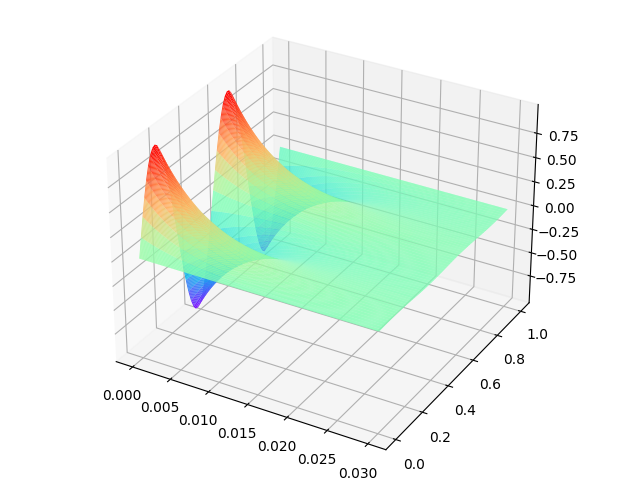
\includegraphics[width=0.45\textwidth]{result_u.png}}
\subfigure[精确解]{
\label{Fig.sub.2}
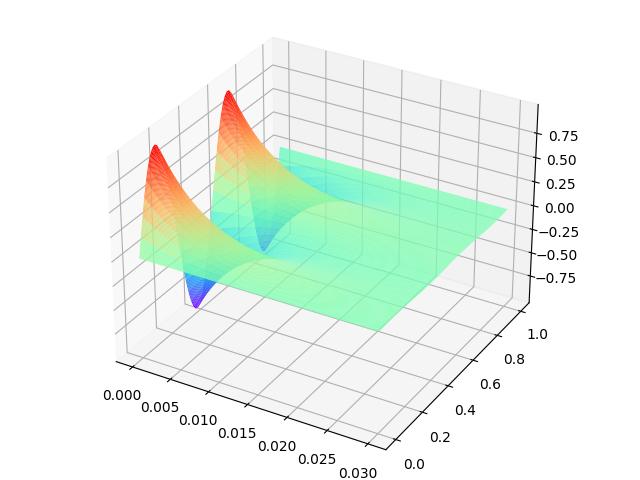
\includegraphics[width=0.45\textwidth]{u_exact.png}}
\caption{$m=320,n=64$结果图}
\label{Fig.main}
\end{figure}

精确解与数值解之差的绝对值$||u-[u]||$如图\ref{Fig.main2},计算得到误差为
$||u-[u]||_c=0.0015189395174771136$。
\begin{figure}[H] %H为当前位置,!htb为忽略美学标准,htbp为浮动图形
    \centering %图片居中
    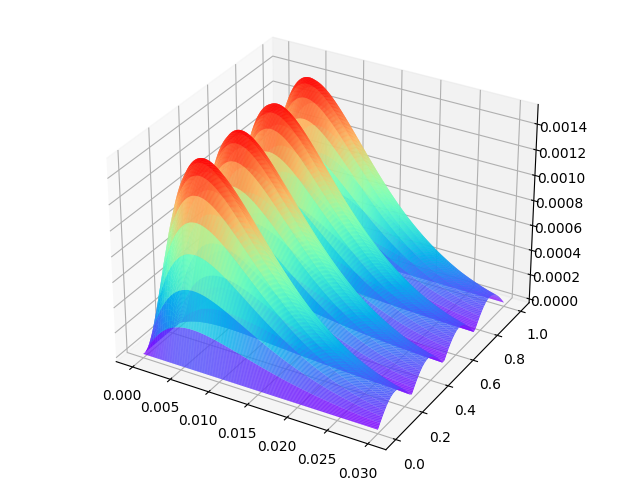
\includegraphics[width=1\textwidth]{abs_error.png} %插入图片,[]中设置图片大小,{}中是图片文件名
    \caption{$||u-[u]||$结果图} %最终文档中希望显示的图片标题
    \label{Fig.main2} %用于文内引用的标签
\end{figure}

当取不同的$\tau,h$时,计算得到的误差如表所示。

\begin{longtable}{cccccc}
    \caption{不同$\tau,h$的误差表}\\\hline
    $\tau$ & $h$ & 误差e &
    \multicolumn{1}{c}{$e_i/e_{i+1}$} \\\hline
    \endfirsthead
    \caption[]{不同$\tau,h$的误差表(续表)}\\
    \multicolumn{4}{r}{\footnotesize 接上页}\\\hline
    $\tau$ & $h$ & 误差err & \multicolumn{1}{c}{$e_i/e_{i+1}$}\\
    \hline\endhead
    \hline\multicolumn{4}{r}{\footnotesize 接下页}\\
    \endfoot\hline\hline\endlastfoot
    $\frac{1}{10}$ & $\frac{1}{10}$ & 0.0428079643162558 &  \\
    $\frac{1}{40}$ & $\frac{1}{20}$ & 0.00951825176096948 & 4.4975\\
    $\frac{1}{160}$ & $\frac{1}{40}$ & 0.00244056613219328 & 3.9000\\
    $\frac{1}{640}$ & $\frac{1}{80}$ & 0.000606385251482932 & 4.0248\\
    $\frac{1}{2560}$ & $\frac{1}{160}$ & 0.000151362159712509 & 4.0062\\
\end{longtable}

我们知道最简显格式的误差为$||[u]^k-u^k||=O(\tau + h^2)$,设$e_i=C \times (\tau_i + h_i^2)$,
取$\tau_{i+1}=\frac{1}{4} \tau_i$,$h_{i+1}=\frac{1}{2}h_i$,可以得到$\frac{e_i}{e_{i+1}}
=4$,与表1结果相符,从而也验证了最简显格式的误差阶数为$O(\tau + h^2)$.
\end{document}